\chapter{平面圆锥曲线}


我从研究圆锥曲线的几何性质开始，作为射影平面 \({\mathbb{P}}^{2}\) 项目的动机.射影几何通常在二年级本科几何课程中提及，这里我将回顾了一些显著特征，着重于齐次坐标，尽管我完全忽略了线性子空间的几何和“交比”等概念.学生最重要的目标应是理解几何思想(例如，“无穷远点”对应曲线的渐近方向)如何用坐标表达.直观几何图像(告诉你应期待什么)与坐标的精确定义(让你能利用直觉)之间的互动，正是代数几何的迷人之处.

\section{参数化曲线示例}

毕达哥拉斯定理指出，在图中

\[
{X}^{2} + {Y}^{2} = {Z}^{2},
\]

\begin{center}
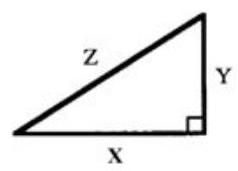
\includegraphics[max width=0.2\textwidth]{images/bo_d3lj80c601uc738kffi0_16_718_1301_238_171_0.jpg}
\end{center}

每个古埃及人都知道，(3,4,5)和(5,12,13)是勾股数.问题是如何找到所有整数解？该方程是齐次的，因此令\(x = X/Z,y = Y/Z\)，它对应着圆\(C : \left( {{x}^{2} + {y}^{2} = 1}\right)  \subset  {\mathbb{R}}^{2}\) ，可以被参数化为

\[
x = \frac{2\lambda }{{\lambda }^{2} + 1},\;y = \frac{{\lambda }^{2} - 1}{{\lambda }^{2} + 1},\;\text{其中}\;\lambda  = \frac{x}{1 - y};
\]

由此可得通解:

\[
X = 2\ell m,\;Y = {\ell }^{2} - {m}^{2},\;Z = {\ell }^{2} + {m}^{2}\;\text{其中}\ell ,m \in  \mathbb{Z}\text{互素}
\]

(如果 \(\ell ,m\) 均为奇数，则各除以2).注意该方程是齐次的，因此如果(X, Y, Z)是解，则 \(\left( {{\lambda X},{\lambda Y},{\lambda Z}}\right)\) 也是解.

也许这个参数化在学校几何中已经熟悉，无论如何，很容易验证它是正确的.然而，如果我之前不知道它，我可以通过一个简单的几何论证得到它，即从给定点的线性射影: \(P = \left( {0,1}\right)  \in  C\) ，如果 \(\lambda  \in  \mathbb{Q}\)
\begin{center}
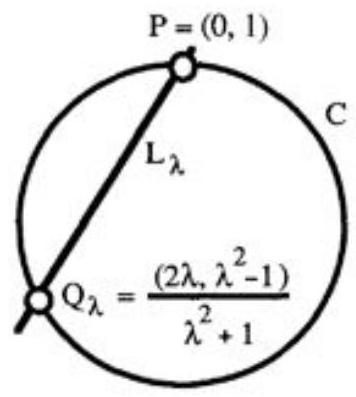
\includegraphics[max width=0.2\textwidth]{images/bo_d3lj80c601uc738kffi0_17_772_501_356_397_0.jpg}
\captionof{figure}{圆锥曲线到直线的线性射影}
\end{center}

是任意值，则通过 \(P\) 且斜率为 \(- \lambda\) 的直线 \({L}_{\lambda }\) 与 \(C\) 相交于另一点 \({Q}_{\lambda }\) .这种通过线性射影构造映射的方法将在后续多次出现.

\section{类似例子}

\(C : \left( {2{X}^{2} + {Y}^{2} = 5{Z}^{2}}\right)\) .同样的方法导出了参数化 \(\mathbb{R} \rightarrow  C\) ，其表达式为

\[
x = \frac{2\sqrt{5}\lambda }{1 + 2{\lambda }^{2}},\;y = \frac{2{\lambda }^{2} - 1}{1 + 2{\lambda }^{2}}.
\]

这使我们能够理解所有系数属于 \(\mathbb{R}\) 的 \(C\) 上的点，且与前一个例子没有实质区别；那么 \(\mathbb{Q}\) 呢？

命题 如果 \(\left( {a,b,c}\right)  \in  \mathbb{Q}\) 满足 \(2{a}^{2} + {b}^{2} = 5{c}^{2}\) ，则 \(\left( {a,b,c}\right)  = \left( {0,0,0}\right)\) .

证明 通过乘以公分母并在必要时提取公因子，我可以假设 \(a,b,c\) 是整数，且不全被5整除；此外，如果 \(5 \mid  a\) 且 \(5 \mid  b\) ，则 \({25} \mid  5{c}^{2}\) ，从而 \(5 \mid  c\) ，这与我刚才所说矛盾.现在通过考虑 \(a\) 和 \(b{\;\operatorname{mod}\;5}\) 的可能取值很容易得到矛盾:由于任何平方数都是0、1或4 \({\;\operatorname{mod}\;5}\) ，显然 \(2{a}^{2} + {b}^{2}\) 是 \(0 + 1,0 + 4,2 + 0,2 + 1,2 + 4,8 + 0,8 + 1\) 或 \(8 + 4{\;\operatorname{mod}\;5}\) 之一，且都不可能是 \(5{c}^{2}\) 的形式.证毕.

注意这是一个彻底的算术论证.

\section{\({\mathbb{R}}^{2}\) 中的圆锥曲线}

\({\mathbb{R}}^{2}\) 中的圆锥曲线是由二次方程给出的平面曲线
\[
q\left( {x,y}\right)  = a{x}^{2} + {bxy} + c{y}^{2} + {dx} + {ey} + f = 0.
\]

每个人都见过非退化圆锥曲线的分类:

\begin{center}
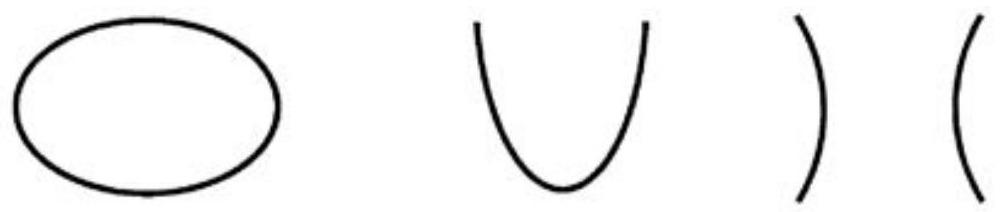
\includegraphics[max width=0.7\textwidth]{images/bo_d3lj80c601uc738kffi0_18_341_562_1004_212_0.jpg}
\captionof{figure}{非退化圆锥曲线:(a) 椭圆；(b) 抛物线；(c) 双曲线.}
\end{center}
\hspace*{3em} 


此外，还有一些特殊情况:

(d) 由 \({x}^{2} + {y}^{2} = 0\) 给出的单点；

(e, f, g) 由以下三个方程中的任意一个给出的空集:(e) \({x}^{2} + {y}^{2} =  - 1\) ，(f) \({x}^{2} =  - 1\) 或 (g) \(0 = 1\) .这三个方程不同，尽管它们在 \({\mathbb{R}}^{2}\) 中定义了相同的零点轨迹；例如考虑它们的复数解.

(h) 直线 \(x = 0\) ；

(i) 直线对 \({xy} = 0\) ；

(j) 平行直线 \(x\left( {x - 1}\right)  = 0\) ；

(k) “重直线” \({x}^{2} = 0\) ；你可以自行决定是否允许最后一种情况:

(l) 由 \(0 = 0\) 给出的整个平面.

\section{射影平面}

“凭空”定义:

\begin{align*}
{\mathbb{P}}^{2}\mathbb{R} &= \left\{{\mathbb{R}}^{3}\text{中经过原点的直线}\right\}\\
&= \{ \text{比例}X : Y : Z\}\\
&= \left( {{\mathbb{R}}^{3}\setminus \{ 0\} }\right) / \sim  ,\;\text{其中}\left( {X,Y,Z}\right)  \sim  \left( {{\lambda X},{\lambda Y},{\lambda Z}}\right),\forall\,\lambda  \in  \mathbb{R} \setminus  \{ 0\} .
\end{align*}

(有经验的读者将轻松地从 \({\mathbb{R}}^{3}\) 推广到任意域上的向量空间，并用内在论证替代选定坐标系中的计算.)

为了表示比值 \(X : Y : Z\) ，其中 \(Z \neq  0\) ，我可以设定 \(x = X/Z,y = Y/Z\) ；这简化了问题，因为该比值对应于仅两个实数.换言之，(X, Y, Z)在 \(\sim\) 下的等价类有唯一代表(x, y,1)，其第三坐标为 \(= 1\) .不幸的是，有时 \(Z\) 可能为 \(= 0\) ，因此这种选择等价类代表的方法就不适用了.这说明 \({\mathbb{P}}^{2}\mathbb{R}\) 包含了 \({\mathbb{R}}^{2}\) 的一个副本.示意图:

\begin{center}
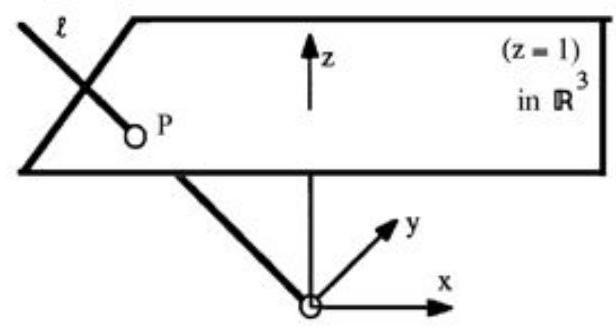
\includegraphics[max width=0.4\textwidth]{images/bo_d3lj80c601uc738kffi0_19_646_280_616_328_0.jpg}
\captionof{figure}{由 \({\mathbb{R}}^{2} \hookrightarrow  {\mathbb{R}}^{3} \setminus  \{ 0\}  \rightarrow  {\mathbb{P}}^{2}\mathbb{R}\) 除以 \(\left( {x,y}\right)  \mapsto  \left( {x,y,1}\right)\)}
\end{center}
\hspace*{3em} 

\({\mathbb{R}}^{3}\) 中通过0的一般直线不包含于平面 \(\left( {Z = 0}\right)\) ，因此它与 \(\left( {Z = 1}\right)\) 恰好相交于一点，该点是该等价类的代表. \(\left( {Z = 0}\right)\) 中的直线永远不与 \(\left( {Z = 1}\right)\) 相交，因此它们对应的不是 \({\mathbb{R}}^{2}\) 的点，而是渐近方向，或 \({\mathbb{R}}^{2}\) 中平行直线簇；所以你可以将 \({\mathbb{P}}^{2}\mathbb{R}\) 视为由 \({\mathbb{R}}^{2}\) 及每个平行直线簇的一个“无穷远点”组成.从这个角度看，你在 \({\mathbb{R}}^{2}\) 中计算，试图通过某种“渐近”论证猜测无穷远处的情况，然后(如有必要)用齐次坐标证明.用 \({\mathbb{R}}^{3}\) 中的直线定义使这一点合理，因为它平等对待了 \({\mathbb{P}}^{2}\mathbb{R}\) 中的所有点.

变换群在整个几何学中具有核心重要性；几何图形的性质必须在适当类型的变换下保持不变，才能具有意义. \({\mathbb{R}}^{2}\) 中的仿射坐标变换形式为 \(T\left( z\right)  = Ax + B\) ，其中 \(x = \left( {x,y}\right)  \in  {\mathbb{R}}^{2}\) ， \(A\) 是一个 \(2 \times  2\) 可逆矩阵， \(B\) 是平移向量；如果 \(A\) 是正交矩阵，则该变换 \(T\) 是欧氏变换.众所周知，每个非退化的圆锥曲线都可以通过欧氏变换化简为上述标准形式(a-c)之一.读者可以尝试证明，每个圆锥曲线都可以通过仿射变换化简为形式(a-1)之一.

\({\mathbb{P}}^{2}\mathbb{R}\) 的射影变换或射影映射是形如 \(T\left( \mathbf{X}\right)  = M\mathbf{X}\) 的映射，其中 \(M\) 是一个可逆的 \(3 \times  3\) 矩阵.理解该变换对仿射部分 \({\mathbb{R}}^{2} \subset  {\mathbb{P}}^{2}\mathbb{R}\) 的作用很简单:作为一个部分定义的映射 \({\mathbb{R}}^{2} \rightarrow  {\mathbb{R}}^{2}\) ，它是分式线性变换.

\[
\left( \begin{array}{l} x \\  y \end{array}\right)  \mapsto  \left( {A\left( \begin{array}{l} x \\  y \end{array}\right)  + B}\right) /\left( {{cx} + {dy} + e}\right) ,\;\text{ where }\;M = \left( \begin{matrix} A & B \\  c & d \end{matrix}\right) .
\]

当 \({cx} + {dy} + e = 0\) 时， \(T\) 当然未定义.或许这看起来不太直观，但它确实存在于自然界:同一(平面)物体的两张不同照片显然通过射影变换相关；参见例如[Berger, 4.7.4]中的图片.因此，一位数学研究生若从事卫星摄影解译工作(无论是为林业委员会的和平目的，还是作为里根总统国防政策带来的广阔职业前景的一部分)，将花费大量时间计算射影变换.

射影变换在这些笔记中隐含使用，通常以“通过适当选择坐标，我可以假设……”的形式出现.

\section{圆锥曲线的方程}

非齐次二次多项式

\[
q\left( {x,y}\right)  = a{x}^{2} + {bxy} + c{y}^{2} + {dx} + {ey} + f
\]

对应于齐次二次多项式

\[
Q\left( {X,Y,Z}\right)  = a{X}^{2} + {bXY} + c{Y}^{2} + {dXZ} + {eYZ} + f{Z}^{2};
\]

这种对应关系易于理解为一种操作步骤，或者你也可以将其视为由 \(q \leftrightarrow  Q\) 给出的双射

\[
q\left( {x,y}\right)  = Q\left( {X/Z,Y/Z,1}\right) \;\text{ with }\;x = X/Z,y = Y/Z
\]

反之亦然，

\[
Q = {Z}^{2}q\left( {X/Z,Y/Z}\right) .
\]

圆锥曲线 \(C \subset  {\mathbb{P}}^{2}\) 是由 \(C : \left( {Q\left( {X,Y,Z}\right)  = 0}\right)\) 给出的曲线，其中 \(Q\) 是一个齐次二次表达式；注意条件 \(Q\left( {X,Y,Z}\right)  = 0\) 在等价类上定义良好，因为对于任意 \(\lambda  \in  \mathbb{R}\) ，有 \(Q\left( {\lambda \mathbf{X}}\right)  = {\lambda }^{2}Q\left( \mathbf{X}\right)\) .作为练习，验证射影曲线 \(C\) 在仿射片 \({\mathbb{R}}^{2}\) 中与由 \(\left( {q = 0}\right)\) 给出的仿射圆锥曲线相交.

\subsection{“无穷远直线”与渐近方向}

\({\mathbb{P}}^{2}\) 中满足 \(Z = 0\) 的点对应于比值 \(\left( {X : Y : 0}\right)\) .这些点构成无穷远直线，是 \({\mathbb{P}}_{\mathbb{R}}^{1} = \mathbb{R} \cup  \{ \infty \}\) 的一个副本(因为 \(\left( {X : Y}\right)  \mapsto  X/Y\) 定义了一个从 \({\mathbb{P}}_{\mathbb{R}}^{1} \rightarrow  \mathbb{R} \cup  \{ \infty \}\) 到 \({\mathbb{P}}_{\mathbb{R}}^{1} = \mathbb{R} \cup  \{ \infty \}\) 的双射).

\({\mathbb{P}}^{2}\) 中的直线定义为由 \(L : \left( {{aX} + {bY} + {cZ} = 0}\right)\) 给出，且

\[
L\text{ passes through }\left( {X,Y,0}\right)  \Leftrightarrow  {aX} + {bY} = 0\text{ . }
\]

在仿射坐标中，同一条直线由 \({ax} + {by} + c = 0\) 给出，因此所有具有相同比例 \(a : b\) 的直线都通过同一个无穷远点.这称为“平行线在无穷远处相交”.

例(a) 双曲线 \(\left( {\frac{{x}^{2}}{{a}^{2}} - \frac{{y}^{2}}{{b}^{2}} = 1}\right)\) 在 \({\mathbb{R}}^{2}\) 中对应于 \({\mathbb{P}}^{2}\mathbb{R}\) 中的 \(C : \left( {\frac{{X}^{2}}{{a}^{2}} - \frac{{Y}^{2}}{{b}^{2}} = {Z}^{2}}\right)\) ；显然它在 \(\left( {Z = 0}\right)\) 中与两点 \(\left( {a, \pm  b,0}\right)  \in  {\mathbb{P}}^{2}\mathbb{R}\) 相交，这两点显然对应于双曲线的渐近线.

注意，在 \({\mathbb{P}}^{2}\mathbb{R}\) 的仿射片 \(\left( {X \neq  0}\right)\) 中，仿射坐标为 \(u = Y/X,v = Z/X\) ，因此 \(C\) 变为椭圆 \(\left( {\frac{{u}^{2}}{{b}^{2}} + {v}^{2} = \frac{1}{{a}^{2}}}\right)\) .参见练习1.7中的艺术性诠释.

(b) 抛物线 \(\left( {y = m{x}^{2}}\right)\) 在 \({\mathbb{R}}^{2}\) 中对应于 \({\mathbb{P}}^{2}\mathbb{R}\) 中的 \(C : \left( {{YZ} = m{X}^{2}}\right)\) ；它现在在单点(0,1,0)处与 \(\left( {Z = 0}\right)\) 相交.因此在 \({\mathbb{P}}^{2}\) 中，“抛物线的两支在无穷远处相遇”；注意这是一条具有直观意义的陈述(也许你觉得这很难以置信？)，但这不是仅凭在 \({\mathbb{R}}^{2} -\) 内的思考就能得出的结论，甚至可能没有意义.

\section{\({\mathbb{P}}^{2}\) 中圆锥曲线的分类}

设 \(k\) 为特征为 \(\neq  2\) 的任意域；回顾二次型线性代数中的两个结果:

命题 (A) 存在自然的双射

\[
\left\{  \begin{matrix} \text{ homogeneous } \\  \text{ quadratic polys. } \end{matrix}\right\}   = \left\{  \begin{matrix} \text{ quad. forms } \\  {k}^{3} \rightarrow  k \end{matrix}\right\}  \overset{\text{ bij }}{ \leftrightarrow  }\left\{  \begin{matrix} \text{ symmetric bilinear } \\  \text{ forms on }{k}^{3} \end{matrix}\right\}
\]

由公式给出

\[
a{X}^{2} + {2bXY} + c{Y}^{2} + {2dXZ} + {2eYZ} + f{Z}^{2} \leftrightarrow  \left( \begin{array}{lll} a & b & d \\  b & c & e \\  d & e & f \end{array}\right)
\]

当对应的双线性型非退化，即其矩阵非奇异时，二次型称为非退化的.

定理 (B) 设 \(V\) 为定义在 \(k\) 上的向量空间， \(Q : V \rightarrow  k\) 为二次型；则存在 \(V\) 的一组基，使得

\[
Q = {\varepsilon }_{1}{x}_{1}^{2} + {\varepsilon }_{2}{x}_{2}^{2} + \cdots  + {\varepsilon }_{n}{x}_{n}^{2},\text{ with }{\varepsilon }_{i} \in  k.
\]

(这通过Gram-Schmidt正交化法证明，如果你还记得的话.)显然，对于 \(\lambda  \in\)  \(k \setminus  \{ 0\}\) ，代换 \({x}_{i} \mapsto  \lambda {x}_{i}\) 将 \({\varepsilon }_{i}\) 变为 \({\lambda }^{-2}{\varepsilon }_{i}\) .

推论 在适当的坐标系中， \({\mathbb{P}}^{2}\mathbb{R}\) 中的任一圆锥曲线为以下之一:

( \(\alpha\) )非退化圆锥曲线， \(C : \left( {{X}^{2} + {Y}^{2} - {Z}^{2} = 0}\right)\) ；

( \(\beta\) )空集，由 \(\left( {{X}^{2} + {Y}^{2} + {Z}^{2} = 0}\right)\) 给出；

(γ)直线对，由 \(\left( {{X}^{2} - {Y}^{2} = 0}\right)\) 给出；

(δ)单点(0,0,1)，由 \(\left( {{X}^{2} + {Y}^{2} = 0}\right)\) 给出；

(ε)重直线，由 \(\left( {{X}^{2} = 0}\right)\) 给出.

(可选地，整个 \({\mathbb{P}}^{2}\mathbb{R}\) 由 \(\left( {0 = 0}\right)\) 给出.)

证明 任意实数 \(\varepsilon\) 要么为0，要么为±平方数，因此我只需考虑定理中 \(Q\) 为 \({\varepsilon }_{i} = 0\) 或 \(\pm  1\) 的情况.此外，由于我只关心轨迹 \(\left( {Q = 0}\right)\) ，允许将 \(Q\) 乘以-1.这立即导出上述列表.证毕.

关于此推论有两点需要说明:首先，该列表比(1.3)中的要短得多；例如，(1.3)中的3种非退化情况(椭圆、抛物线、双曲线)均对应于 \(\left( \alpha \right)\) 情况，而相交和平行直线对在射影情况下未加区分.其次，该列表从一般代数原理推导出来更为简洁.

\section{1.7 圆锥曲线的参数化}

设 \(C\) 为 \({\mathbb{P}}^{2}\mathbb{R}\) 中一个非退化且非空的圆锥曲线.则根据推论1.6，取新坐标后， \(\left( {X + Z,Y,Z - X}\right) ,C\) 与曲线 \(\left( {{XZ} = {Y}^{2}}\right)\) 在射影意义下等价；该曲线由下式参数化

\[
\Phi  : {\mathbb{P}}_{\mathbb{R}}^{1} \rightarrow  C \subset  {\mathbb{P}}^{2}\mathbb{R}
\]

\[
\left( {U : V}\right)  \mapsto  \left( {{U}^{2} : {UV} : {V}^{2}}\right) .
\]

备注1 逆映射 \(\Psi  : C \rightarrow  {\mathbb{P}}_{\mathbb{R}}^{1}\) 由下式给出

\[
\left( {X : Y : Z}\right)  \mapsto  \left( {X : Y}\right)  = \left( {Y : Z}\right) ;
\]

此处左侧的比值在 \(X \neq  0\) 时定义，右侧的比值在 \(Z \neq  0\) 时定义.用稍后引入的术语， \(\Phi\) 和 \(\Psi\) 是簇的逆同构.

2 在整个 \(§§1 - 2\) 中，默认非空非退化圆锥曲线在射影意义下等价于 \(\left( {{XZ} - {Y}^{2}}\right)\) ；在特征为 \(\neq  2\) 的域上，这一点在练习1.5中得到了证明.(对特征2感兴趣的读者应将此作为非退化圆锥曲线的定义.)

\section{1.8 两变量齐次形式}

设 \(F\left( {U,V}\right)\) 为 \(U,V\) 中一个次数为 \(d\) 的非零齐次多项式，系数属于固定域 \(k\) ；(我将沿用传统，使用“形式”一词表示“齐次多项式”):

\[
F\left( {U,V}\right)  = {a}_{d}{U}^{d} + {a}_{d - 1}{U}^{d - 1}V + \cdots  + {a}_{i}{U}^{i}{V}^{d - i} + \cdots  + {a}_{0}{V}^{d}.
\]

\(F\) 对应一个一元非齐次多项式，

\[
f\left( u\right)  = {a}_{d}{u}^{d} + {a}_{d - 1}{u}^{d - 1} + \cdots  + {a}_{i}{u}^{i} + \cdots  + {a}_{0}.
\]

显然对于 \(\alpha  \in  k\) ，

\[
f\left( \alpha \right)  = 0 \Leftrightarrow  \left( {u - \alpha }\right)  \mid  f\left( u\right)
\]

\[
\Leftrightarrow  \left( {U - {\alpha V}}\right)  \mid  F\left( {U,V}\right)  \Leftrightarrow  F\left( {\alpha ,1}\right)  = 0;
\]

因此 \(f\) 的零点对应于 \({\mathbb{P}}^{1}\) 上除点(1,0)——即“点 \(\alpha  = \infty\) ”外的 \(F\) 的零点. \(F\) 在无穷远点有零点意味着什么？

\[
F\left( {1,0}\right)  = 0 \Leftrightarrow  {a}_{d} = 0 \Leftrightarrow  \deg f < d.
\]

现定义 \(F\) 在 \({\mathbb{P}}^{1}\) 上的零点的重数为

(i) 对应于 \(\alpha  \in  k\) 处 \(f\) 的重数；或

(ii) 若零点为(1,0)，则为 \(d - \deg f\) .

因此， \(F\) 在点 \(\left( {\alpha ,1}\right)\) 处的零点重数是整除 \(F\) 的最大 \(\left( {U - {\alpha V}}\right)\) 次幂，而在(1,0)处则是整除 \(F\) 的最大 \(V\) 次幂.

命题 设 \(F\left( {U,V}\right)\) 为 \(U,V\) 中次数为 \(d\) 的非零形式.则 \(F\) 在 \({\mathbb{P}}^{1}\) 上最多有 \(d\) 个零点；此外，若 \(k\) 是代数闭域，则 \(F\) 在 \({\mathbb{P}}^{1}\) 上恰有 \(d\) 个零点，前提是这些零点按上述定义的重数计数.

证明 设 \({m}_{\infty }\) 为 \(F\) 在(1,0)处零点的重数；则根据定义， \(d - {m}_{\infty }\) 是非齐次多项式 \(f\) 的次数，命题归结为一元多项式最多有 \(\deg f\) 个根的众所周知的事实.证毕.

注意，在代数闭域上， \(F\) 可分解为线性形式 \({\lambda }_{i} = \left( {{a}_{i}U + {b}_{i}V}\right)\) 的乘积 \(F = \prod {\lambda }_{i}^{{m}_{i}}\) ，以此方式处理时，点(1,0)对应形式 \({\lambda }_{\infty } = V\) ，与其他点处于同等地位.

\section{Bézout定理的简单情形}

Bézout定理指出，如果 \(C\) 和 \(D\) 是次数分别为 \(\deg C = m,\deg D = n\) 的平面曲线，那么它们的交点数为 \({mn}\) ，前提是(i)域是代数闭合的；(ii)交点按正确的重数计数；(iii)我们在 \({\mathbb{P}}^{2}\) 中工作，以正确考虑“无穷远处”的交点.详见例如[Fulton，第112页]的自包含证明.本节将讨论其中一条曲线为直线或圆锥曲线的情况.

定理 设 \(L \subset  {\mathbb{P}}_{k}^{2}\) 为一条直线(分别为 \(C \subset  {\mathbb{P}}_{k}^{2}\) 一条非退化圆锥曲线)，且设 \(D \subset  {\mathbb{P}}_{k}^{2}\) 为由 \(D : \left( {{G}_{d}\left( {X,Y,Z}\right)  = 0}\right)\) 定义的曲线，其中 \(G\) 是 \(X,Y,Z\) 中次数为 \(d\) 的齐次多项式.假设 \(L ⊄ D\) (分别为 \(C ⊄ D\) )；则

\[
\# \{ L \cap  D\}  \leq  d\;\text{ (respectively }\# \{ C \cap  D\}  \leq  {2d}\text{ ). }
\]

事实上，存在一个自然的交点重数定义，使得不等式对“按重数计数的点数”仍然成立，且如果 \(k\) 是代数闭合的，则等号成立.

证明 一条直线 \(L \subset  {\mathbb{P}}_{k}^{2}\) 由方程 \(\lambda  = 0\) 给出，其中 \(\lambda\) 是线性形式；为方便起见，我用参数形式表示为

\[
X = a\left( {U,V}\right) ,\;Y = b\left( {U,V}\right) ,\;Z = c\left( {U,V}\right) ,
\]

其中 \(a,b,c\) 是 \(U,V\) 中的线性形式.例如，如果 \(\lambda  = {\alpha X} + {\beta Y} + {\gamma Z}\) ，且 \(\gamma  \neq  0\) ，则 \(L\) 可以

表示为

\[
X = U,\;Y = V,\;Z =  - \frac{\alpha }{\gamma }U - \frac{\beta }{\gamma }V.
\]

类似地，如(1.7)所述，非退化圆锥曲线可以参数化表示为

\[
X = a\left( {U,V}\right) ,\;Y = b\left( {U,V}\right) ,\;Z = c\left( {U,V}\right) ,
\]

其中 \(a,b,c\) 是 \(U,V\) 中的二次形式.这是因为 \(C\) 是 \(\left( {{XZ} = {Y}^{2}}\right)\) 的射影变换，而 \(\left( {{XZ} = {Y}^{2}}\right)\) 的参数形式为 \(\left( {X,Y,Z}\right)  = \left( {{U}^{2},{UV},{V}^{2}}\right)\) ，因此 \(C\) 由下式给出

\[
\left( \begin{array}{l} X \\  Y \\  Z \end{array}\right)  = M\left( \begin{matrix} {U}^{2} \\  {UV} \\  {V}^{2} \end{matrix}\right)
\]

其中 \(M\) 是一个非奇异的 \(3 \times  3\) 矩阵.

\begin{center}
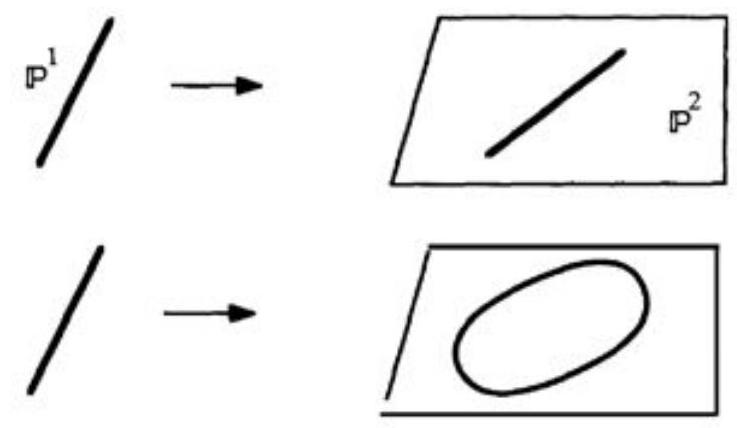
\includegraphics[max width=0.5\textwidth]{images/bo_d3lj80c601uc738kffi0_24_454_273_737_428_0.jpg}
\end{center}
\hspace*{3em} 

图1.4:(a)参数化直线；(b)参数化圆锥曲线

那么 \(L\) (分别为 \(C\) )与 \(D\) 的交点由求解比值 \(\left( {U : V}\right)\) 的值确定，使得

\[
F\left( {U,V}\right)  = {G}_{d}\left( {a\left( {U,V}\right) ,b\left( {U,V}\right) ,c\left( {U,V}\right) }\right)  = 0.
\]

但 \(F\) 是 \(U,V\) 中次数为 \(d\) (分别为 \({2d}\) )的齐次多项式，故结果由(1.8)得出.证毕.

\setboxcounter{corollary}{9}
\begin{corollary}\label{cor:1.10}
    若 \({P}_{1},\ldots ,{P}_{5} \in  {\mathbb{P}}^{2}\mathbb{R}\) 为不同点且无四点共线，则最多存在一条经过 \({P}_{1},\ldots ,{P}_{5}\) 的圆锥曲线.ss
\end{corollary}

\begin{proof}
    反设 \({C}_{1}\) 和 \({C}_{2}\) 为圆锥曲线，且 \({C}_{1} \neq  {C}_{2}\) 使得

\[
{C}_{1} \cap  {C}_{2} \supset  \left\{  {{P}_{1},\ldots ,{P}_{5}}\right\}
\]

\({C}_{1}\) 非空，则若其非退化，则由(1.7)知其在射影意义下等价于参数化曲线

\[
{C}_{1} = \left\{  {\left( {{U}^{2},{UV},{V}^{2}}\right)  \mid  \left( {U,V}\right)  \in  {\mathbb{P}}^{1}}\right\}  ;
\]
由 \(\left( {1.9}\right) ,{C}_{1} \subset  {C}_{2}\) .现在如果 \({Q}_{2}\) 是 \({C}_{2}\) 的方程，则对于所有 \(\left( {U,V}\right)  \in  {\mathbb{P}}^{1}\) 都有 \({Q}_{2}\left( {{U}^{2},{UV},{V}^{2}}\right)  \equiv  0\) ，且一个简单的计算(见练习1.6)表明 \({Q}_{2}\) 是 \(\left( {{XZ} - {Y}^{2}}\right)\) 的倍数；这与 \({C}_{1} \neq  {C}_{2}\) 矛盾.

现在假设 \({C}_{1}\) 是退化的；根据(1.6)，它要么是一对直线，要么是一条直线，很容易看出

\[
{C}_{1} = {L}_{0} \cup  {L}_{1},\;{C}_{2} = {L}_{0} \cup  {L}_{2},
\]

其中 \({L}_{1},{L}_{2}\) 是不同的直线.则 \({C}_{1} \cap  {C}_{2} = {L}_{0} \cup  \left( {{L}_{1} \cap  {L}_{2}}\right)\) :

\begin{center}
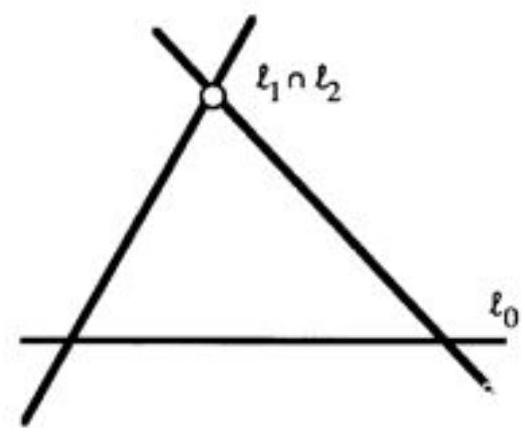
\includegraphics[max width=0.4\textwidth]{images/bo_d3lj80c601uc738kffi0_25_718_284_525_437_0.jpg}
\captionof{figure}{相交的直线}
\end{center}
\hspace*{3em} 



因此 \({P}_{1},\ldots ,{P}_{5}\) 中的4个点位于 \({L}_{0}\) 上，矛盾.
\end{proof}


\setcounter{section}{10}
\section{所有圆锥曲线的空间}

设

\[
{S}_{2} = \left\{  {\text{ quadratic forms on }{\mathbb{R}}^{3}}\right\}   = \{ 3 \times  3\text{ symmetric matrixes }\}  \cong  {\mathbb{R}}^{6}.
\]

如果 \(Q \in  {S}_{2}\) ，写作 \(Q = a{X}^{2} + {2bXY} + \cdots  + f{Z}^{2}\) ；对于 \({P}_{0} = \left( {{X}_{0},{Y}_{0},{Z}_{0}}\right)  \in  {\mathbb{P}}^{2}\mathbb{R}\) ，考虑关系 \({P}_{0} \in  C : \left( {Q = 0}\right)\) .这具有以下形式

\[
Q\left( {{X}_{0},{Y}_{0},{Z}_{0}}\right)  = a{X}_{0}^{2} + {2b}{X}_{0}{Y}_{0} + \cdots  + f{Z}_{0}^{2} = 0,
\]

对于固定的 \({P}_{0}\) ，这是关于 \(\left( {a,b,\ldots ,f}\right)\) 的线性方程.因此

\[
{S}_{2}\left( {P}_{0}\right)  = \left\{  {Q \in  {S}_{2} \mid  Q\left( {P}_{0}\right)  = 0}\right\}   \cong  {\mathbb{R}}^{5} \subset  {S}_{2} = {\mathbb{R}}^{6}
\]

是一个5维超平面.对于 \({P}_{1},\ldots ,{P}_{n} \in  {\mathbb{P}}^{2}\mathbb{R}\) ，类似定义

\[
{S}_{2}\left( {{P}_{1},\ldots ,{P}_{n}}\right)  = \left\{  {Q \in  {S}_{2} \mid  Q\left( {P}_{i}\right)  = 0\text{ for }i = 1,\ldots ,n}\right\}  ;
\]

则在 \(Q\) 的6个系数 \(\left( {a,b,\ldots ,f}\right)\) 中有 \(n\) 个线性方程.由此得到结果:

命题 \(\dim {S}_{2}\left( {{P}_{1},\ldots ,{P}_{n}}\right)  \geq  6 - n\) .

我们还可以预期“当 \({P}_{1},\ldots ,{P}_{n}\) 足够一般时等号成立”.更准确地说:

推论 如果 \(n \leq  5\) 且 \({P}_{1},\ldots ,{P}_{n}\) 中没有4点共线，则

\[
\dim {S}_{2}\left( {{P}_{1},\ldots ,{P}_{n}}\right)  = 6 - n.
\]

证明 推论1.10表明如果 \(n = 5\) ，则 \(\dim {S}_{2}\left( {{P}_{1},\ldots ,{P}_{5}}\right)  \leq  1\) ，这在此情况下给出推论.如果 \(n \leq  4\) ，则我可以加入点 \({P}_{n + 1},\ldots ,{P}_{5}\) ，同时保持没有4点共线的条件，且由于每个点最多施加一个线性条件，这给出

\[
1 = \dim {S}_{2}\left( {{P}_{1},\ldots ,{P}_{5}}\right)  \geq  \dim {S}_{2}\left( {{P}_{1},\ldots ,{P}_{n}}\right)  - \left( {5 - n}\right) \text{ . Q.E.D. }
\]

注意，如果给定6个点 \({P}_{1},\ldots ,{P}_{6} \in  {\mathbb{P}}^{2}\mathbb{R}\) ，它们可能在圆锥曲线上，也可能不在.

\section{1.12 两条圆锥曲线的交点}

如上所述，两条圆锥曲线常常在4个点相交:

\begin{center}
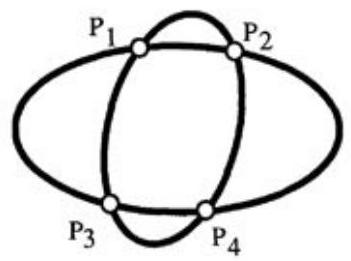
\includegraphics[max width=0.2\textwidth]{images/bo_d3lj80c601uc738kffi0_26_669_694_351_261_0.jpg}
\end{center}
\hspace*{3em} 

反过来，根据推论1.11，给定4个点 \({P}_{1},\ldots ,{P}_{4} \in  {\mathbb{P}}^{2}\) ，在适当条件下 \({S}_{2}\left( {{P}_{1},\ldots ,{P}_{4}}\right)\) 是一个二维向量空间，因此选择 \({S}_{2}\left( {{P}_{1},\ldots ,{P}_{4}}\right)\) 的基 \({Q}_{1},{Q}_{2}\) 会得到两条圆锥曲线 \({C}_{1},{C}_{2}\) ，使得 \({C}_{1} \cap  {C}_{2} = \left\{  {{P}_{1},\ldots ,{P}_{4}}\right\}\) .非奇异圆锥曲线多重交点有多种可能:

\begin{center}
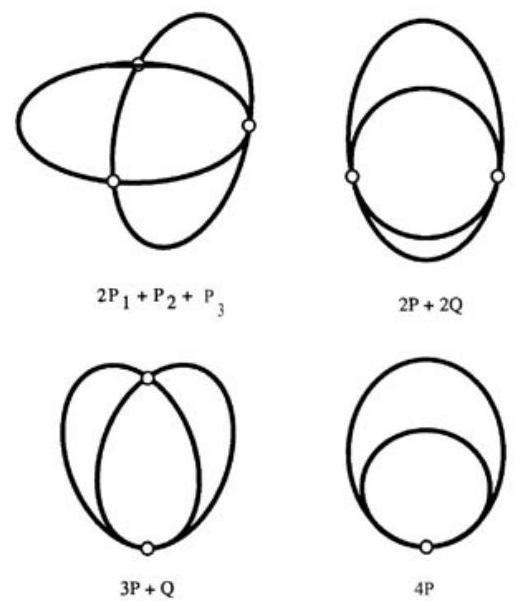
\includegraphics[max width=0.4\textwidth]{images/bo_d3lj80c601uc738kffi0_26_578_1167_519_608_0.jpg}
\end{center}
\hspace*{3em} 

图1.6:(a) \(2{P}_{1} + {P}_{2} + {P}_{3}\) ；(b) \({2P} + {2Q}\) ；(c) \({3P} + Q\) ；(d) \({4P}\)

参见练习1.9获取合适的方程.

\section{1.13 圆锥曲线族中的退化圆锥曲线}

定义 圆锥曲线族(pencil of conics)是形如

\[
{C}_{\left( \lambda ,\mu \right) } : \left( {\lambda {Q}_{1} + \mu {Q}_{2} = 0}\right) ;
\]

的族，每个元素都是平面曲线，线性依赖于参数 \(\left( {\lambda ,\mu }\right)\) ；将比值 \(\left( {\lambda  : \mu }\right)\) 视为 \({\mathbb{P}}^{1}\) 上的一点.

观察示例，可以预期当 \(\left( {\lambda  : \mu }\right)\) 取特殊值时，圆锥曲线 \({C}_{\left( \lambda ,\mu \right) }\) 会退化.事实上，记对应二次型 \(Q\) 的对称矩阵 \(3 \times  3\) 的行列式为 \(\det \left( Q\right)\) ，则显然

\[
{C}_{\left( \lambda ,\mu \right) }\text{ is degenerate } \Leftrightarrow  \det \left( {\lambda {Q}_{1} + \mu {Q}_{2}}\right)  = 0\text{ . }
\]

将 \({Q}_{1}\) 和 \({Q}_{2}\) 写成对称矩阵形式，条件可表达为

\[
F\left( {\lambda ,\mu }\right)  = \det \left| {\lambda \left( \begin{array}{lll} a & b & d \\  b & c & e \\  d & e & f \end{array}\right)  + \mu \left( \begin{array}{lll} {a}^{\prime } & {b}^{\prime } & {d}^{\prime } \\  {b}^{\prime } & {c}^{\prime } & {e}^{\prime } \\  {d}^{\prime } & {e}^{\prime } & {f}^{\prime } \end{array}\right) }\right|  = 0.
\]

注意 \(F\left( {\lambda ,\mu }\right)\) 是关于 \(\lambda ,\mu\) 的齐次三次型.进而我可以对 \(F\) 应用(1.8)推导出:

命题 设 \({C}_{\left( \lambda ,\mu \right) }\) 是 \({\mathbb{P}}_{k}^{2}\) 上的一个圆锥曲线族，且至少包含一个非退化圆锥曲线(即 \(F\left( {\lambda ,\mu }\right)\) 不恒为零).则该族最多有3个退化圆锥曲线.如果 \(k = \mathbb{R}\) ，则该族至少有一个退化圆锥曲线.

证明 三次型有 \(\leq  3\) 个零点.在 \(\mathbb{R}\) 上，它至少有一个零点.

\section{1.14 例题解析}

设 \({P}_{1},\ldots ,{P}_{4}\) 是 \({\mathbb{P}}^{2}\mathbb{R}\) 中的4个点，且无3点共线；则通过 \({P}_{1},\ldots ,{P}_{4}\) 的圆锥曲线族 \({C}_{\left( \lambda ,\mu \right) }\) 有3个退化元素，即线对 \({L}_{12} + {L}_{34},{L}_{13} + {L}_{24},{L}_{14} + {L}_{23}\) ，其中 \({L}_{ij}\) 是通过 \({P}_{i},{P}_{j}\) 的直线:

\begin{center}
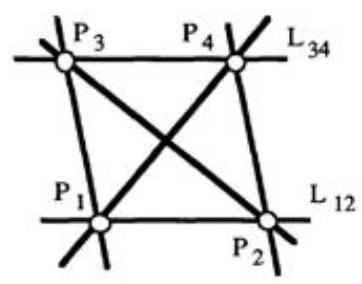
\includegraphics[max width=0.2\textwidth]{images/bo_d3lj80c601uc738kffi0_27_770_1529_362_284_0.jpg}
\end{center}
\hspace*{3em} 

接下来，假设我从由 \({Q}_{1} = {Y}^{2} + {rY} + {sX} + t\) 和 \({Q}_{2} = Y - {X}^{2}\) 生成的圆锥曲线族出发，尝试找到交点 \({P}_{1},\ldots ,{P}_{4}\) .

\begin{center}
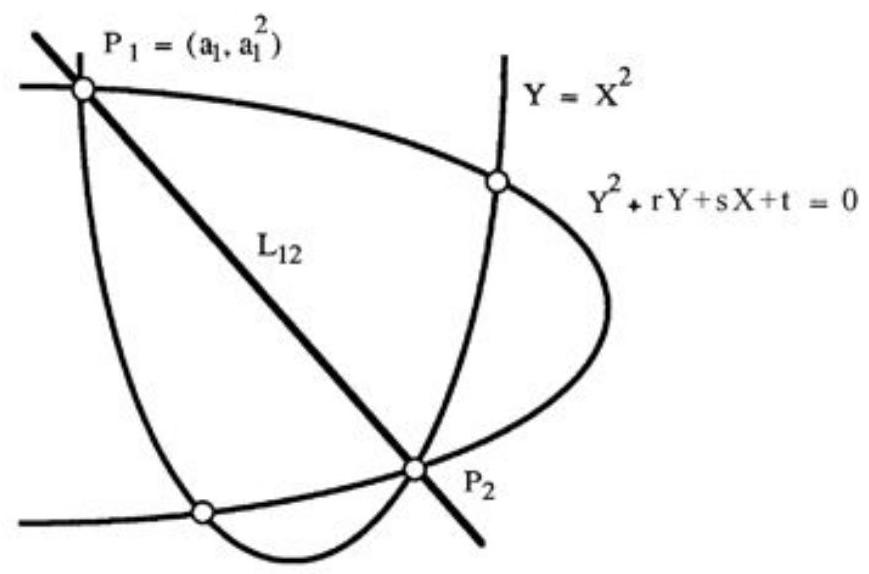
\includegraphics[max width=0.6\textwidth]{images/bo_d3lj80c601uc738kffi0_28_418_286_869_574_0.jpg}
\end{center}
\hspace*{3em} 

这可以按如下方式完成:(1) 找到使 \({C}_{\left( \lambda ,\mu \right) }\) 成为退化圆锥曲线的3个比率 \(\left( {\lambda  : \mu }\right)\) .根据上述内容，这仅意味着我必须找到该三次方程的3个根

\[
F\left( {\lambda ,\mu }\right)  = \det \left| {\lambda \left( \begin{matrix} 0 & 0 & s/2 \\  0 & 1 & r/2 \\  s/2 & r/2 & t \end{matrix}\right)  + \mu \left( \begin{matrix}  - 1 & 0 & 0 \\  0 & 0 & 1/2 \\  0 & 1/2 & 0 \end{matrix}\right) }\right|
\]

\[
=  - \frac{1}{4}\left( {{s}^{2}{\lambda }^{3} + \left( {{4t} - {r}^{2}}\right) {\lambda }^{2}\mu  - {2r\lambda }{\mu }^{2} - {\mu }^{3}}\right) .
\]

(2) 将其中2个退化圆锥曲线分解为直线对(这涉及解2个二次方程).(3) 4个点 \({P}_{i}\) 是这些直线的交点.

该过程为伽罗瓦理论(Galois theory)中一般四次方程的约化提供了几何解释(参见例如[van der Waerden, Algebra, 第8章, \(§{64}\) ]):设 \(k\) 为一个域， \(f\left( X\right)  =\)  \({X}^{4} + r{X}^{2} + {sX} + t \in  k\left\lbrack  X\right\rbrack\) 为一个四次多项式.则两条抛物线 \({C}_{1}\) 和 \({C}_{2}\) 在4个点 \({P}_{i} = \left( {{a}_{i},{a}_{i}^{2}}\right)\) 相交，其中 \(i = 1,\ldots ,4\) ，而 \({a}_{i}\) 是 \(f\) 的4个根.

则直线 \({L}_{ij} = {P}_{i}{P}_{j}\) 由下式给出

\[
{L}_{ij} : \left( {Y = \left( {{a}_{i} + {a}_{j}}\right) X - {a}_{i}{a}_{j}}\right) ,
\]

而可约圆锥曲线 \({L}_{12} + {L}_{34}\) 由下式给出

\[
{Y}^{2} + \left( {{a}_{1}{a}_{2} + {a}_{3}{a}_{4}}\right) Y + \left( {{a}_{1} + {a}_{2}}\right) \left( {{a}_{3} + {a}_{4}}\right) {X}^{2} + {sX} + t = 0,
\]

即由 \({Q}_{1} - \left( {{a}_{1} + {a}_{2}}\right) \left( {{a}_{3} + {a}_{4}}\right) {Q}_{2} = 0\) 给出.因此，使圆锥曲线 \(\lambda {Q}_{1} + \mu {Q}_{2}\) 分解为直线对的3个 \(\mu /\lambda\) 值为

\[
- \left( {{a}_{1} + {a}_{2}}\right) \left( {{a}_{3} + {a}_{4}}\right) ,\; - \left( {{a}_{1} + {a}_{3}}\right) \left( {{a}_{2} + {a}_{4}}\right) ,\; - \left( {{a}_{1} + {a}_{4}}\right) \left( {{a}_{2} + {a}_{3}}\right) .
\]

这些3个量作为根的三次方程称为与四次方程相关的辅助三次方程；它可以通过初等对称函数理论计算；这是一个相当繁琐的过程.另一方面，上述几何方法给出了辅助三次方程的优雅推导，仅涉及计算一个 \(3 \times  3\) 行列式.

上述处理摘自[M.Berger, 16.4.10 和 16.4.11.1].

\section{第一章习题}

1.1 通过考虑经过点(2,1)的变量直线对圆锥曲线 \(C : \left( {{x}^{2} + {y}^{2} = 5}\right)\) 进行参数化，从而求出 \({x}^{2} + {y}^{2} = 5\) 的所有有理解.

1.2 设 \(p\) 为素数；通过对不同的 \(p\) 进行实验，猜测 \({x}^{2} + {y}^{2} = p\) 存在有理解的充要条件；证明你的猜测(提示见下文习题1.9之后

\begin{itemize}
\item 打赌你自己做不到！).
\end{itemize}

1.3 证明(1.3)中的陈述，即仿射变换可用于将任意 \({\mathbb{R}}^{2}\) 的圆锥曲线化为标准形式之一(a-l).【提示:使用线性变换 \(\mathbf{x} \mapsto  A\mathbf{x}\) 将首项 \(a{x}^{2} + {bxy} + c{y}^{2}\) 变换为 \(\pm  {x}^{2} \pm  {y}^{2}\) 或 \(\pm  {x}^{2}\) 或0；然后对 \(x\) 和 \(y\) 完成平方，尽可能消除线性部分.】

1.4 详细比较(1.3)中的仿射圆锥曲线与(1.6)中的射影圆锥曲线.

1.5 设 \(k\) 为特征为 \(\neq  2\) 的任意域， \(V\) 为三维 \(k\) -向量空间；设 \(Q : V \rightarrow  k\) 为 \(V\) 上的非退化二次型.证明若 \(0 \neq  {e}_{1} \in  V\) 满足 \(Q\left( {e}_{1}\right)  = 0\) ，则 \(V\) 存在基 \({e}_{1},{e}_{2},{e}_{3}\) 使得 \(Q\left( {{x}_{1}{e}_{1} + {x}_{2}{e}_{2} + {x}_{3}{e}_{3}}\right)  = {x}_{1}{x}_{3} + a{x}_{2}^{2}\) .【提示:考虑与 \(Q\) 相关的对称双线性型 \(\varphi\) ；由于 \(\varphi\) 非退化，存在向量 \({e}_{3}\) 使得 \(\varphi \left( {{e}_{1},{e}_{3}}\right)  = 1\) .然后找到合适的 \({e}_{2}\) .】

推断非空且非退化的圆锥曲线 \(C \subset  {\mathbb{P}}_{k}^{2}\) 在射影意义下等价于 \(({XZ} =\)  \(\left. {Y}^{2}\right)\) .

1.6 设 \(k\) 为元素数不少于4的域，且 \(C : \left( {{XZ} = {Y}^{2}}\right)  \subset  {\mathbb{P}}_{k}^{2}\) ；证明若 \(Q\left( {X,Y,Z}\right)\) 为在 \(C\) 上消失的二次型，则 \(Q = \lambda \left( {{XZ} - {Y}^{2}}\right)\) .【提示:如果你确实无法自行完成，可参照引理2.5证明中的论证.】

1.7 在 \({\mathbb{R}}^{3}\) 中，考虑两个平面 \(A : \left( {Z = 1}\right)\) 和 \(B : \left( {X = 1}\right)\) ；一条通过0点的直线在 \(A\) 上交于(x, y,1)，在 \(B\) 上交于 \(\left( {1,y/x,1/x}\right)\) .考虑由 \(\left( {x,y}\right)  \mapsto  \left( {y}^{\prime }\right.  =\)  \(\left. {y/x,{z}^{\prime } = 1/x}\right)\) 定义的映射 \(\varphi  : A \rightarrow  B\) ；求 \(\varphi\) 下的像

(i) 直线 \({ax} = y + b\) ；平行线束 \({ax} = y + b\) (固定 \(a\) ，变化 \(b\) )；

(ii) 对于变化的 \(c\) ，圆 \({\left( x - 1\right) }^{2} + {y}^{2} = c\) (区分三种情况 \(c > 1,c = 1\) 和 \(c < 1\) ).

试想象上述内容为一位坐在 \(0 \in  {\mathbb{R}}^{3}\) 上的艺术家，在平面 \(\left( {X = 1}\right)\) 上对平面 \(\left( {Z = 1}\right)\) 上的图形所作的透视画.解释当 \(\varphi\) 和 \({\varphi }^{-1}\) 未定义时，两平面上的点会发生什么变化.

1.8 设 \({P}_{1},\ldots ,{P}_{4}\) 为 \({\mathbb{P}}^{2}\) 中不共线的不同点，且无三点共线.证明存在唯一的坐标系，使得这4点为 \(\left( {1,0,0}\right) ,\left( {0,1,0}\right) ,\left( {0,0,1}\right)\) 和(1,1,1).找出所有经过 \({P}_{1},\ldots ,{P}_{5}\) 的圆锥曲线，其中 \({P}_{5} = \left( {a,b,c}\right)\) 为另一点，并用此给出推论1.10和命题1.11的另一证明.

1.9 在(1.12)中列出了两条圆锥曲线相交的所有可能方式.写出方程证明每种可能确实存在.找出对应线束中所有奇异圆锥曲线.[提示:利用对称性和恰当选择的坐标系可大大简化计算.]

1.2的提示:根据初等数论，-1是模 \(p\) 的二次剩余当且仅当 \(p = 2\) 或 \(p \equiv  1{\;\operatorname{mod}\;4}\) .

1.10(Sylvester行列式).设 \(k\) 为代数闭域，且在 \(U,V\) 中给定二次型和三次型，如(1.8)所示:

\[
q\left( {U,V}\right)  = {a}_{0}{U}^{2} + {a}_{1}{UV} + {a}_{2}{V}^{2},
\]

\[
c\left( {U,V}\right)  = {b}_{0}{U}^{3} + {b}_{1}{U}^{2}V + {b}_{2}U{V}^{2} + {b}_{3}{V}^{3}.
\]

证明 \(q\) 和 \(c\) 有公共零点 \(\left( {\eta  : \tau }\right)  \in  {\mathbb{P}}^{1}\) 当且仅当

\[
\det \left| \begin{array}{lllll} {a}_{0} & {a}_{1} & {a}_{2} & & \\   & {a}_{0} & {a}_{1} & {a}_{2} & \\   & & {a}_{0} & {a}_{1} & {a}_{2} \\  {b}_{0} & {b}_{1} & {b}_{2} & {b}_{3} & \\   & {b}_{0} & {b}_{1} & {b}_{2} & {b}_{3} \end{array}\right|  = 0
\]

[提示:证明若 \(q\) 和 \(c\) 有公共根，则这5个元素

\[
{U}^{2}q,\;{UVq},\;{V}^{2}q,\;{Uc}\;\text{ and }\;{Vc}
\]

不生成4次型的5维向量空间，因此线性相关.反之，利用多项式环 \(k\left\lbrack  {U,V}\right\rbrack\) 中的唯一分解性质，说明形如 \({Aq} = {Bc}\) 的关系，其中 \(A\) 和 \(B\) 为 \(U,V,\deg A = 2,\deg B = 1\) 中的形式.

1.11 将练习1.10的结果推广到 \(U,V\) 中任意次数为 \(n\) 和 \(m\) 的两个形式.